\subsection{Finite Element Method}

\subsubsection{General Idea}
Problems involving the calculations of electromagnetic fields are often cumbersome and difficult to solve. This is due to the need of solving differential equations describing these fields over a computational domain, which is not possible with a computer in this sense. The simulation software Ansys HFSS (High Frequency Simulation Software) aims to provide a solution. This software is used for the simulations in \autoref{sec:simulations}, hence it is described in this following, dedicated section.

HFSS uses a numerical technique, namely the Finite Element Method (FEM). The general idea of FEM after Rayleigh-Ritz-Galerkin is to choose a number of basis functions. The goal is to find a linear combination of these basis functions, so that the differential equation is satisfied as closely as possible. This turns the problem of solving a differential equation into a system of algebraic equations, which the computer can process. There is always a set of basis functions which enable the calculation to converge to the real solution. However, the number of basis functions used in the domain is limited, due to reasons of computability \cite{STRANG_2018}. 

FEM therefore divides the domain into finite elements, i.e. smaller pieces. Then, within each piece, such a basis function is assigned. A linear combination of these basis functions are found, which satisfy the differential equations. In region where the approximating solution has a high degree of error, the accuracy may be increased by further subdividing the finite elements. This is repeated, until the error falls below a certain threshold, and a precise solution is derived.

\subsubsection{Dividing a computational domain into finite elements}

The differential equation to be solved is shown in \autoref{eqn:full_wave_equation}, where $\epsilon_r$ is the relative permeability and $\mu_r$ is the relative permeability of the material. The variable $k_0$ is the wave number of free space and equals $k_0=\omega\sqrt{\epsilon_0\mu_0}$. \cite{Cendes_Lee_1988,85399,Cendes_1991}.

\begin{equation}
    \nabla\times\left(\frac{1}{\mu_r}\nabla\times\mathbf{E}\right)-k_0^2\epsilon_r\mathbf{E}=0 \quad\text{in $\Omega$}
    \label{eqn:full_wave_equation}
\end{equation}

This equation is solved in a computational domain $\Omega$. This computational domain is divided into finite elements, called a mesh. Each node in this mesh has polynomial functions assigned, which are weighted to approximate the real solution. It has been proven that tetrahedral finite elements are best suited for this task, as they are geometrically flexible and make the definition of complete polynomial approximation functions possible \cite{Shenton_Cendes_1985}. Ansys HFSS uses a adaptive finite element mesh generator, which automatically provides a mesh for a given 3-dimensional construction. The Delaunay tesselation for three-dimensions is used for generating a mesh. It efficiently creates a mesh from objects of arbitrary shapes. Any boundary condition can be added recursively to the mesh. At the heart of this algorithm lies the property, that the circumsphere of an tetrahedra's vertices may not contain other tetrahedra's vertices. 

\autoref{fig:tetrahedral_mesh} shows one of such tetrahedrons. At the edge points, the components of the field which are normal to the respective edge and tangential to the face of the element is stored. At the vertex points, the component of a field which are tangential to the edges are stored. The value of the field at any midpoint is derived through interpolation from the node values. The basis function is used for interpolation.

\begin{figure}[h]
    \centering
    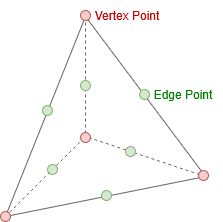
\includegraphics[width=0.25\linewidth]{Documentation/content/10_theory/img/tetrahedral_mesh.png}
    \caption{Tetrahedron with points on the edge and vertices.}
    \label{fig:tetrahedral_mesh}
\end{figure}

Because of the way how the fields are stored in the tetrahedra, they are called tangetial vector finite elements. Their advantage is that tangential components of fields can be forced to be equal among adjacent tetrahedra at the boundary. For example, an electric field stored at a vertex point must point in the direction along one of the edges, therefore it is tangential to the element. An adjacent element then has the same tangential electric field imposed at this node, leading to a continuous tangential electric field, therefore satisfying the boundary conditions implied by the Maxwell equation automatically. Furthermore, any Dirichlet boundary conditions can easily be set along the edges.
\cite{85399}. 

The finite element is described as \autoref{eqn:finite_element_3d}, where $L_2(\Omega)$ is a set of square integrable functions and $P_1$ a set of piecewise linear functions in the discretized domain $\Omega$ \cite{104986}. The vector fields at the vertices are given as $u$. $D(\Omega)$ is a set of divergence free functions. The vectors $u$ used in the finite element therefore 

\begin{itemize}
    \item are continuous in the normal direction.
    \item are square integrable.
    \item have a curl describable by piecewise linear functions.
\end{itemize}

\begin{equation}
    H^{(\dim=3)}_1(\mathrm{curl}) = \left\{ \mathbf{u} \mid \mathbf{u} \in \left[ L_2(\Omega) \right]^3, \nabla \times \mathbf{u} \in \left[ P_1(\Omega) \right]^3 \cap D(\Omega) \right\}
    \label{eqn:finite_element_3d}
\end{equation}

\autoref{fig:tetrahedra_w_unknowns} shows the finite element with the unknowns marked at each point. For reasons of simplicity, only the face is shown. The variables $u_i^j$ and $u_j^i$ are imposed across element boundaries, therefore guaranteeing tangential continuity at boundaries. Additionally, they inherently defined a linear polynomial, meaning that they describe a gradient of the field along this edge. \autoref{eqn:tangential_vector_component} describes this relation mathematically, where $\mathbf{t}_{ij}$ is the unit vector tangentially to the edge from node i to node j and $l_{ij}$ is the length of this edge.

\begin{equation}
    \mathbf{u}\cdot\mathbf{t}_{ij}=\frac{1}{l_{ij}}\left( u_i^j-u_j^i \right)
    \label{eqn:tangential_vector_component}
\end{equation}

\begin{figure}[h]
    \centering
    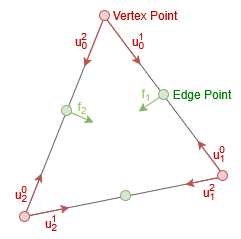
\includegraphics[width=0.25\linewidth]{Documentation//content//10_theory/tetrahedra_w_unknowns.png}
    \caption{Face of the finite element with unknowns}
    \label{fig:tetrahedra_w_unknowns}
\end{figure}

Two facial unknowns $f_1$ and $f_2$ are added to two of the three edge points at one face. Contrary to the variables $u_i^j$, the facial unknowns $f_i$ are only assigned locally at each element and do not cross boundaries. The purpose of the facial unknowns $f$ is to provide a quadratic polynomial for the field component normal to the edges. This will lead to a linear approximation for the curl of the unknown vector field $\nabla\times \mathbf{u}$, providing sufficient accuracy. The overall vector field of this element is then calculated by a superposition of all nodes' vector attributions.

\subsubsection{Solving the differential equation}

A testing function $\mathbf{W}_n$ is defined, which is multiplied to \autoref{eqn:full_wave_equation}. Integrating over the whole test volume then leads to \autoref{eqn:test_funct}. This yields $N$ equations, with $n=1,2,...N$, for each finite element in the domain $\Omega$. This is a common procedure in FEM, and it works through orthogonalization of the residual of \autoref{eqn:full_wave_equation} with respect to the function $\mathbf{W}_n$. This means the new goal of the solution is to minimize the residual by making $\mathbf{W}_n$ as orthogonal as possible \cite{Mohsen_1982}.

\begin{equation}
    \int_\Omega\left( \mathbf{W}_n\cdot\nabla \times\left( \frac{1}{\mu_r}\nabla\times\mathbf{E} \right)-k_0^2\epsilon_r\mathbf{W}_n\cdot\mathbf{E} \right)\mathrm{d}V=0
    \label{eqn:test_funct}
\end{equation}

Using the vector identity $\nabla\cdot\left(\mathbf{a}\times\mathbf{b}\right)=\left(\nabla\times\mathbf{a}\right)\cdot\mathbf{b}-\mathbf{a}\cdot\left(\nabla\times\mathbf{b}\right)$  on \autoref{eqn:test_funct} provides a weak form of the equation, meaning a form of the original partial differential equation, which does not contain all original derivatives \cite{Cendes_Lee_1988,Cendes_1991}. Additionally, boundary terms come into play, as seen in the right hand side of the resulting \autoref{eqn:greens_theorem_wave_eqn}. The usefulness in this step has been described as lowering the highest-order derivative, therefore the approximating functions need to guarantee continuity of value, not of slope \cite{huebner2001finite}. Another explanation is the possibility of incorporation of Neumann boundary conditions \cite{Mohsen_1982}. 

\begin{equation}
    \int_\Omega \left[ \left(\nabla \times \mathbf{W}_n \right)\cdot \frac{1}{\mu_r}\nabla\times \mathbf{E}-k_0^2\epsilon_r\mathbf{W}_n\cdot\mathbf{E}\right]\mathrm{d}V=\underbrace{\oint_{\partial\Omega}\left( \mathbf{W}_n\times \frac{1}{\mu_r}\nabla\times\mathbf{E}\right)\cdot\mathrm{d}\mathbf{S}}_{\text{Boundary term}}
    \label{eqn:greens_theorem_wave_eqn}
\end{equation}

Next, the electric field $\mathbf{E}$ is represented by a superposition of basis functions. When applying Galerkin's method, the basis functions are equal to the test functions $W_n$. \autoref{eqn:representation_e_field_fem} demonstrates the sum of the basis functions, which are weighted with the variable $x_m$. These variables $x$ for all elements have to be solved, to find the electric field $\mathbf{E}$ over the whole domain. The FEM has therefore reduced the initial wave equation in \autoref{eqn:full_wave_equation} to a simple linear matrix equation $Ax=b$, where $A$ is a known $N\times N$ matrix, $b$ contains port excitations and $x$ is the unknown. Ideally, the basis functions are defined to be zero outside of their adjacent elements. This will result to zero for all entries in the matrix, where the test and basis function do not overlap. Therefore, the matrix is sparse, and will be solved much faster. In the end, other electromagnetic quantities can all be derived through the electric field.

\begin{equation}
    \mathbf{E}=\sum^N_mx_m\mathbf{W}_n
    \label{eqn:representation_e_field_fem}
\end{equation}

\autoref{eqn:matrix_a} shows what the matrix then looks like. Some manipulation on the boundary term have been made, so that it contains the surface impedance $Z_s$. The surface impedance defines the ratio of the electric field to the magnetic field on the boundary region. Furthermore, it contains the free space, which equals $\eta_0 \approx 377\,\Omega$.

\begin{equation}
A_{ij} = \int_{\Omega} \nabla \times \mathbf{W}_i \, \frac{1}{\mu_r} \nabla \times \mathbf{W}_j \, \mathrm{d}V 
- k_0^2 \int_{\Omega} \mathbf{W}_i \, \varepsilon_r \mathbf{W}_j \, \mathrm{d}V 
+ \mathrm{i} k_0 \left(\frac{\eta_0}{Z_s}\right) \oint_{\partial\Omega} \mathbf{n} \times \mathbf{W}_i \cdot \mathbf{n} \times \mathbf{W}_j \, \mathrm{d}\mathbf{S}
\label{eqn:matrix_a}
\end{equation}

\subsubsection{Adaptive solution process}

Each finite element therefore has a solved electric field assigned, which should approximate the real solution as closely as possible. To determine the error for each element, \autoref{eqn:full_wave_equation} is evaluated. The elements with the highest residuals contain the largest deviation from the real result, meaning they have a large degree of error. Region in the mesh with large degrees of errors are refined, i.e. the tetrahedral finite elements are split into smaller ones. This allows the FEM solver to recalculate the fields in this region with higher precision, leading to a smaller residual. Consequently, the finite elements represent the fields more accurately, due to a smaller element size and higher resolution \cite{1063929}. An additional method is increasing the order of the polynomial basis functions of elements with low degree of accuracy.

\begin{equation}
    \nabla\times\left(\frac{1}{\mu_r}\nabla\times\mathbf{E}_{\mathrm{solved}}\right)-k_0^2\epsilon_r\mathbf{E}_{\mathrm{solved}}=residual
    \label{eqn:full_wave_equation_solved}
\end{equation}

To determine when the iterative refinement process is done and the solution good enough, some kind of threshold must be defined. One possibility is the $\mathrm{Max}\ \Delta \mathrm{S}$ parameter. It is compared to the difference of S-parameters of the defined excitation ports over two iterations. If, after a mesh refinement, the S-parameters of the ports do not significantly change anymore, meaning change less than $\mathrm{Max}\ \Delta \mathrm{S}$, then the iterative process can be considered done. This described iterative process is shown in \autoref{fig:workflow_fem}. 

\begin{figure}[h]
    \centering
    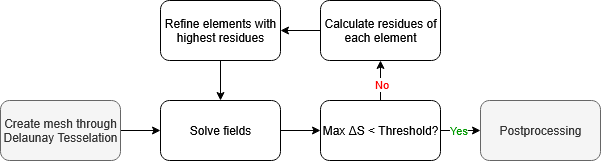
\includegraphics[width=0.75\linewidth]{Documentation//content//20_antennas//img/workflow_fem.png}
    \caption{Adaptive solution process}
    \label{fig:workflow_fem}
\end{figure}

\todo{Short HFSS introduction with boundary conditions, ports and modal and terminal solutions}
 % Fehlende Ressourcen von Zoltan in Journal of Applied Physics. Schreibe über mathetmaische Grundlagen, Meshing, Dipole Excitation und Impedance Network Boundary Counditions (INBC)

% Additional missing ressource: Finite Elements, Electromagnetics, and Design


